\documentclass[12pt]{article}
\usepackage{amsmath}
\usepackage{amssymb}
\usepackage{geometry}
\usepackage{enumerate}
\usepackage{natbib}
\usepackage{float}%稳定图片位置
\usepackage{graphicx}%画图
\usepackage[english]{babel}
\usepackage{a4wide}
\usepackage{indentfirst}%缩进
\usepackage{enumerate}%加序号
\usepackage{multirow}%合并行
\title{\large UM-SJTU JOINT INSTITUTE\\DISCRETE MATHEMATICS\\(VE203)\\\ \\\ \\\ \\\ \\\ \\\ \\\ \\\ \\\ \\\ \\\
ASSIGNMENT 2\\\ \\\ \\\ \\\ \\\ \\\ }
\author{Name: Pan Chongdan\\ID: 516370910121}
\date{Date: \today}


\begin{document}
\maketitle
\newpage
\section{Q1}
\begin{figure}[H]
\centering
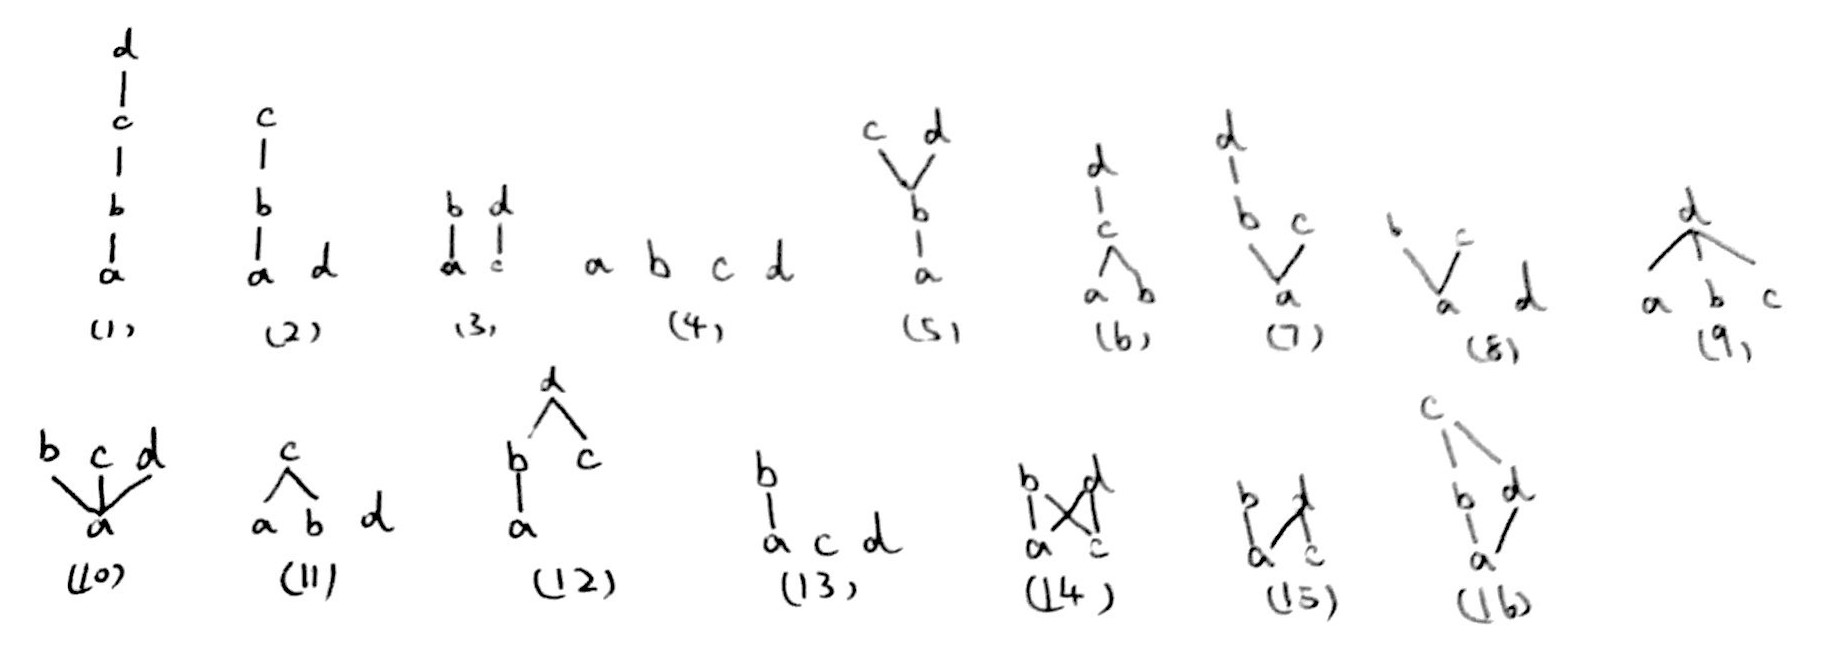
\includegraphics[scale=0.3]{P1.jpg}
\end{figure}
These are 16 possible diagrams of possible partial order. They're all chain complete. The first poset is a linear order and a well order. The 1, 	16 posets are lattices and complete lattices.	
\section{Q2}
\begin{enumerate}[(i)]
\item
If the complete lattice has many maximal elements, then the set of these maximal elements doesn't have a least upper bound, so it can't be a complete lattice.
\item
$$(R,\le)$$
\item
$\forall x\in [a,b],x\leq x\Rightarrow (\mathbb{R},\leq)$ is reflexive.
\\$\forall x,y\in [a,b]$,if $x\leq y$ since $x\neq y\Rightarrow y\nleq x,$
\\$\therefore(\mathbb{R},\leq)$ is antisymmetric.
\\$\forall x,y,z\in [a,b]$,$(x\leq y)\wedge(y\leq z)\Rightarrow(x\leq z),$ 
\\$\therefore(\mathbb{R},\leq)$ is transitive.
\\$\therefore(\mathbb{R},\leq)$ is a poset.
\par $\forall M\subseteq$ if $M$ has one biggest element then it is the least upper bound.
\\if $M$ doesn't have the biggest element and it's an open interval (c,d) $(d\leq b)$, then d is the least upper bound.
\\if $M$ neither has a biggest element and be a interval, then $b$ is its least upper bound.
\\$\therefore M$ must has a least upper bound, similarly it also has a greatest lower bound.
\\$\therefore(\mathbb{R},\leq)$ is a complete lattice. 
\item
$$(\mathbb{N},\ge)$$
\end{enumerate}
\section{Q3}
\begin{figure}[H]
\centering
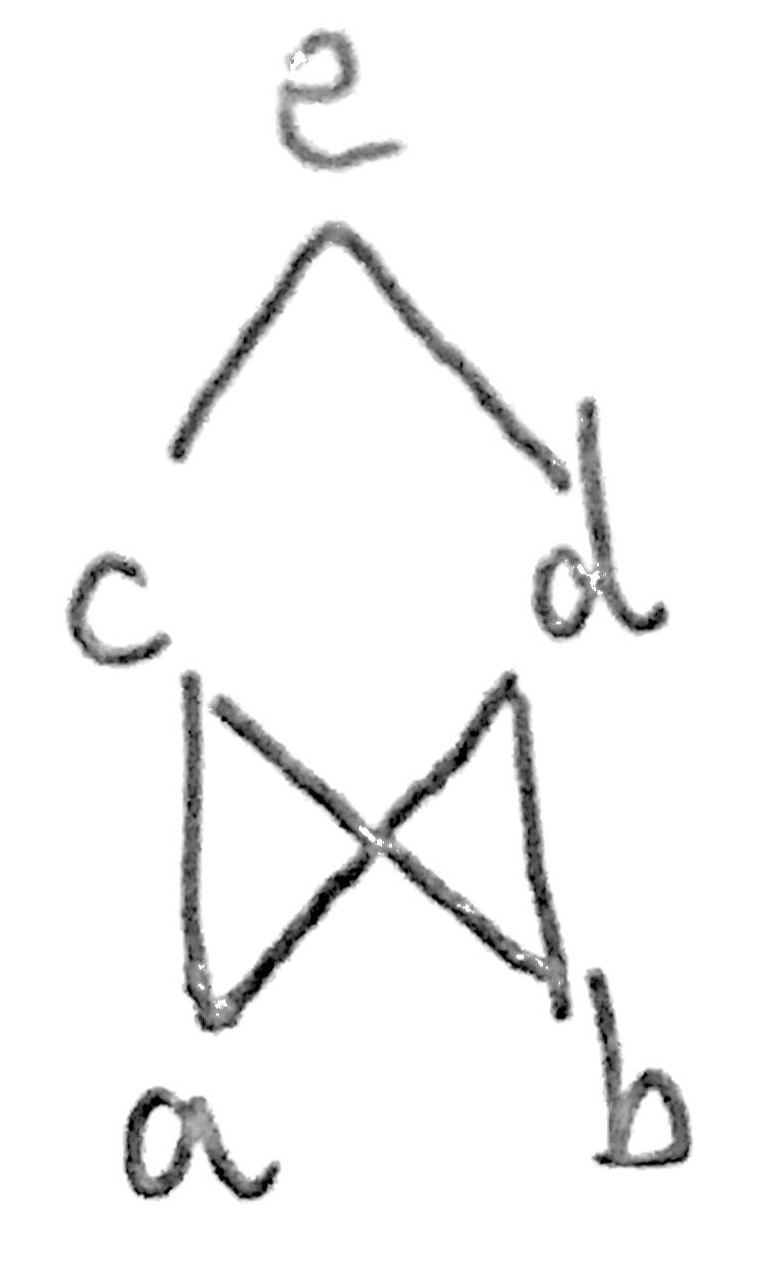
\includegraphics[scale=0.1]{P2.jpg}
\caption{Example of Q3}
\end{figure}
\section{Q4}
$\forall (a,b),(c,d)\in(\mathbb{N}\times\mathbb{N})$
if$(a,b)\npreceq(c,d)$then$((a=c)\wedge (b>d))\vee (a>c)$
\\ $\Rightarrow c<a$ or $(c=a$ and $d\leq b)\Rightarrow(c,d)\preceq(a,b)$
\\ $\therefore (\mathbb{N}\times\mathbb{N},\preceq)$ is a linear order.
\par $(\mathbb{N}\times\mathbb{N},\preceq)$ is well order.
\\$\forall A\subseteq\mathbb{N}\times\mathbb{N}$,assume $A=\mathbb{X}\times\mathbb{Y}$. Since $(\mathbb{N},\leq)$ is a well-order ,then there must exist $x_0\in\mathbb{X}$ and $y_0\in\mathbb{Y}$ such that only $x_0\leq x_0$ and $y_0\leq y_0$. 
\\$\forall[(x,y)\in A]\wedge [(x,y)\neq(x_0,y_0)]\Rightarrow(x_0\leq x)\wedge (y_0\leq y)$ 
\\if$(x>x_0)$ then $(x,y)\npreceq(x_0,y_0)$
\\if$(x=x_0)\wedge(y>y_0)$ then $(x,y)\npreceq(x_0,y_0)$
\\$\therefore$ only $(x_0,y_0)\preceq(x_0,y_0)$ and $(\mathbb{N}\times\mathbb{N},\preceq)$ is a well order.
\section{Q5}
$\forall (a,b)\in(\mathbb{N}\times\mathbb{N}) (a,b)\preceq(a,b)$
\\$\therefore$ it is reflective.
\\if$(a,b)\preceq (c,d)$ then $(a\leq c)\wedge (b\leq d)$
\\Since $(a,b)\neq(c,d)$ $\therefore(c,d)\npreceq(a,b)$ and it's antisymmetric.
\\if$(c,d)\preceq (e,f)$ then $(c\leq e)\wedge (d\leq f)$
\\$\Rightarrow(a\leq e)\wedge (b\leq f)\Rightarrow(a,b)\preceq(e,f)$ and it's transitive.
$\therefore(\mathbb{N}\times\mathbb{N},\preceq)$ is a poset. 
\par It's not a linear order because $(1,3)\npreceq(2,2)$ and $(2,2)\npreceq(1,3)$
\par $\forall (a,b),(c,d)\in(\mathbb{N}\times\mathbb{N}),(max(a,c),max(b,d))$ is the l.u.b and $(min(a,c),min(b,d))$ is the g.l.b.
$\therefore$ It's a lattice.
\section{Q6}
For $(3,3,3),(1,4,4),(2,2,2)\in(\mathbb{Q}\times\mathbb{Q}\times\mathbb{Q}),(3,3,3)\preceq(1,4,4)$ because $3\leq 4,(1,4,4\preceq(2,2,2)$ because $1\leq 2$ but $(3,3,3)\npreceq(1,4,4), \therefore$ it's not transitive and it's not a poset.
\section{Q7}
$\sim$ is equivalence relation
\\$f(x)=f(x)\Rightarrow x\sim x\Rightarrow \sim$ is reflexive
\\$x\sim y\Rightarrow f(x)=f(y)\Rightarrow f(y)=f(x)\Rightarrow y\sim x\Rightarrow \sim$ is symmetric
\\$(x\sim y)\wedge(y\sim z)\Rightarrow(f(x)=f(y))\wedge(f(y)=f(z))$
\\$\Rightarrow f(x)=f(z)\Rightarrow x\sim z\Rightarrow\sim$ is transitive
\\$\therefore \sim$ is equivalence relation 
\par Since $f: A\rightarrow B$ is function, $\forall x_0\in A$, there only exists one $f(x_0)$.
\\$g([x_0]_{\sim})=f(x_0)$
\\$\therefore g$ is a function because f is a function, only $([x_0]_{\sim},f(x_0))\in g$. 
\par $\forall f(x_0)\in B,[x_0]_{\sim}=\{x|(x\in A)\wedge(f(x)=f(x_0))\}$  
\\If $g$ is not injective, then there must exist $[x_1]_{\sim}\neq[x_0]_{\sim}$ such that $g([x_1]_\sim)=f(x_0)$
\\$g([x_1]_\sim)=f(x_1)\Rightarrow f(x_0)=f(x_1)\Rightarrow x_0\sim x_1\Rightarrow [x_0]_\sim=[x_1]_\sim$
It's a contradiction. $\therefore g$ is injective.
\par $f(x)=x^3-4x^2-15x+18=0\Rightarrow x_1=6,x_2=1,x_3=-3$
\\$\therefore g^{-1}(0)=\{6,1,-3\}$
\end{document}